%!TEX program = xelatex

\documentclass{beamer}
\usetheme{metropolis}

\setbeamercolor{background canvas}{bg = white}

\usepackage{appendixnumberbeamer}
\renewcommand\appendixname{Appendix}

% packages
\usepackage{amssymb}
\usepackage{amsmath}
\usepackage{mathtools}
\usepackage{hyperref}
\usepackage{lmodern}

% graphics
\graphicspath{ {Figures/} }

\title{Queues with a Dynamic Schedule}
\author{John Gilbertson}
\date{October 2016}

\begin{document}

\begin{frame}
	\titlepage
\end{frame}

\begin{frame}
	\frametitle{Outline}
	\tableofcontents
\end{frame}

\section{Background}

\begin{frame}
	\frametitle{Queues with Scheduled Arrivals}

	\begin{itemize}
		\item System where customers queue for service
		\item 
	\end{itemize}
\end{frame}

\begin{frame}
	\frametitle{Assumptions}

	\begin{itemize}
		\item Single server
		\item Service times are independent exponential RVs with mean $\mu$
		\item All customers arrive punctually
		\item Total number of customers is fixed
	\end{itemize}
\end{frame}

\begin{frame}
	\frametitle{Static vs. Dynamic}

	\begin{itemize}
		\item 
	\end{itemize}
\end{frame}

\begin{frame}
	\frametitle{Literature Review}

	\begin{itemize}
		\item 
	\end{itemize}
\end{frame}

\section{Static Schedules}

\begin{frame}
	\frametitle{Objective Function}

	\begin{itemize}
		\item Denote the expected waiting time of customer $i$ by $w_{i}$
		\begin{equation*}
			\mathbb{E} \Big[ \text{total customers' waiting time} \Big] = \sum_{i = 1}^{n} w_{i}
		\end{equation*}
		\item Denote the interarrival time between customer $i$ and customer $i + 1$ by $x_{i}$
		\begin{equation*}
			\mathbb{E} \Big[ \text{server availability time} \Big] = \sum_{i = 1}^{n - 1} x_{i} + w_{n} + \mu
		\end{equation*}
		\item Objective is to minimise a linear combination of these times
		\begin{equation*}
			\phi (\mathbf{x}) = (1 - \gamma) \sum_{i = 1}^{n} w_{i} + \gamma \left( \sum_{i = 1}^{n - 1} x_{i} + w_{n} + \mu \right)
		\end{equation*}
	\end{itemize}
\end{frame}

\begin{frame}
	\frametitle{Model for 15 Customers}

	\begin{figure}
			\centering
			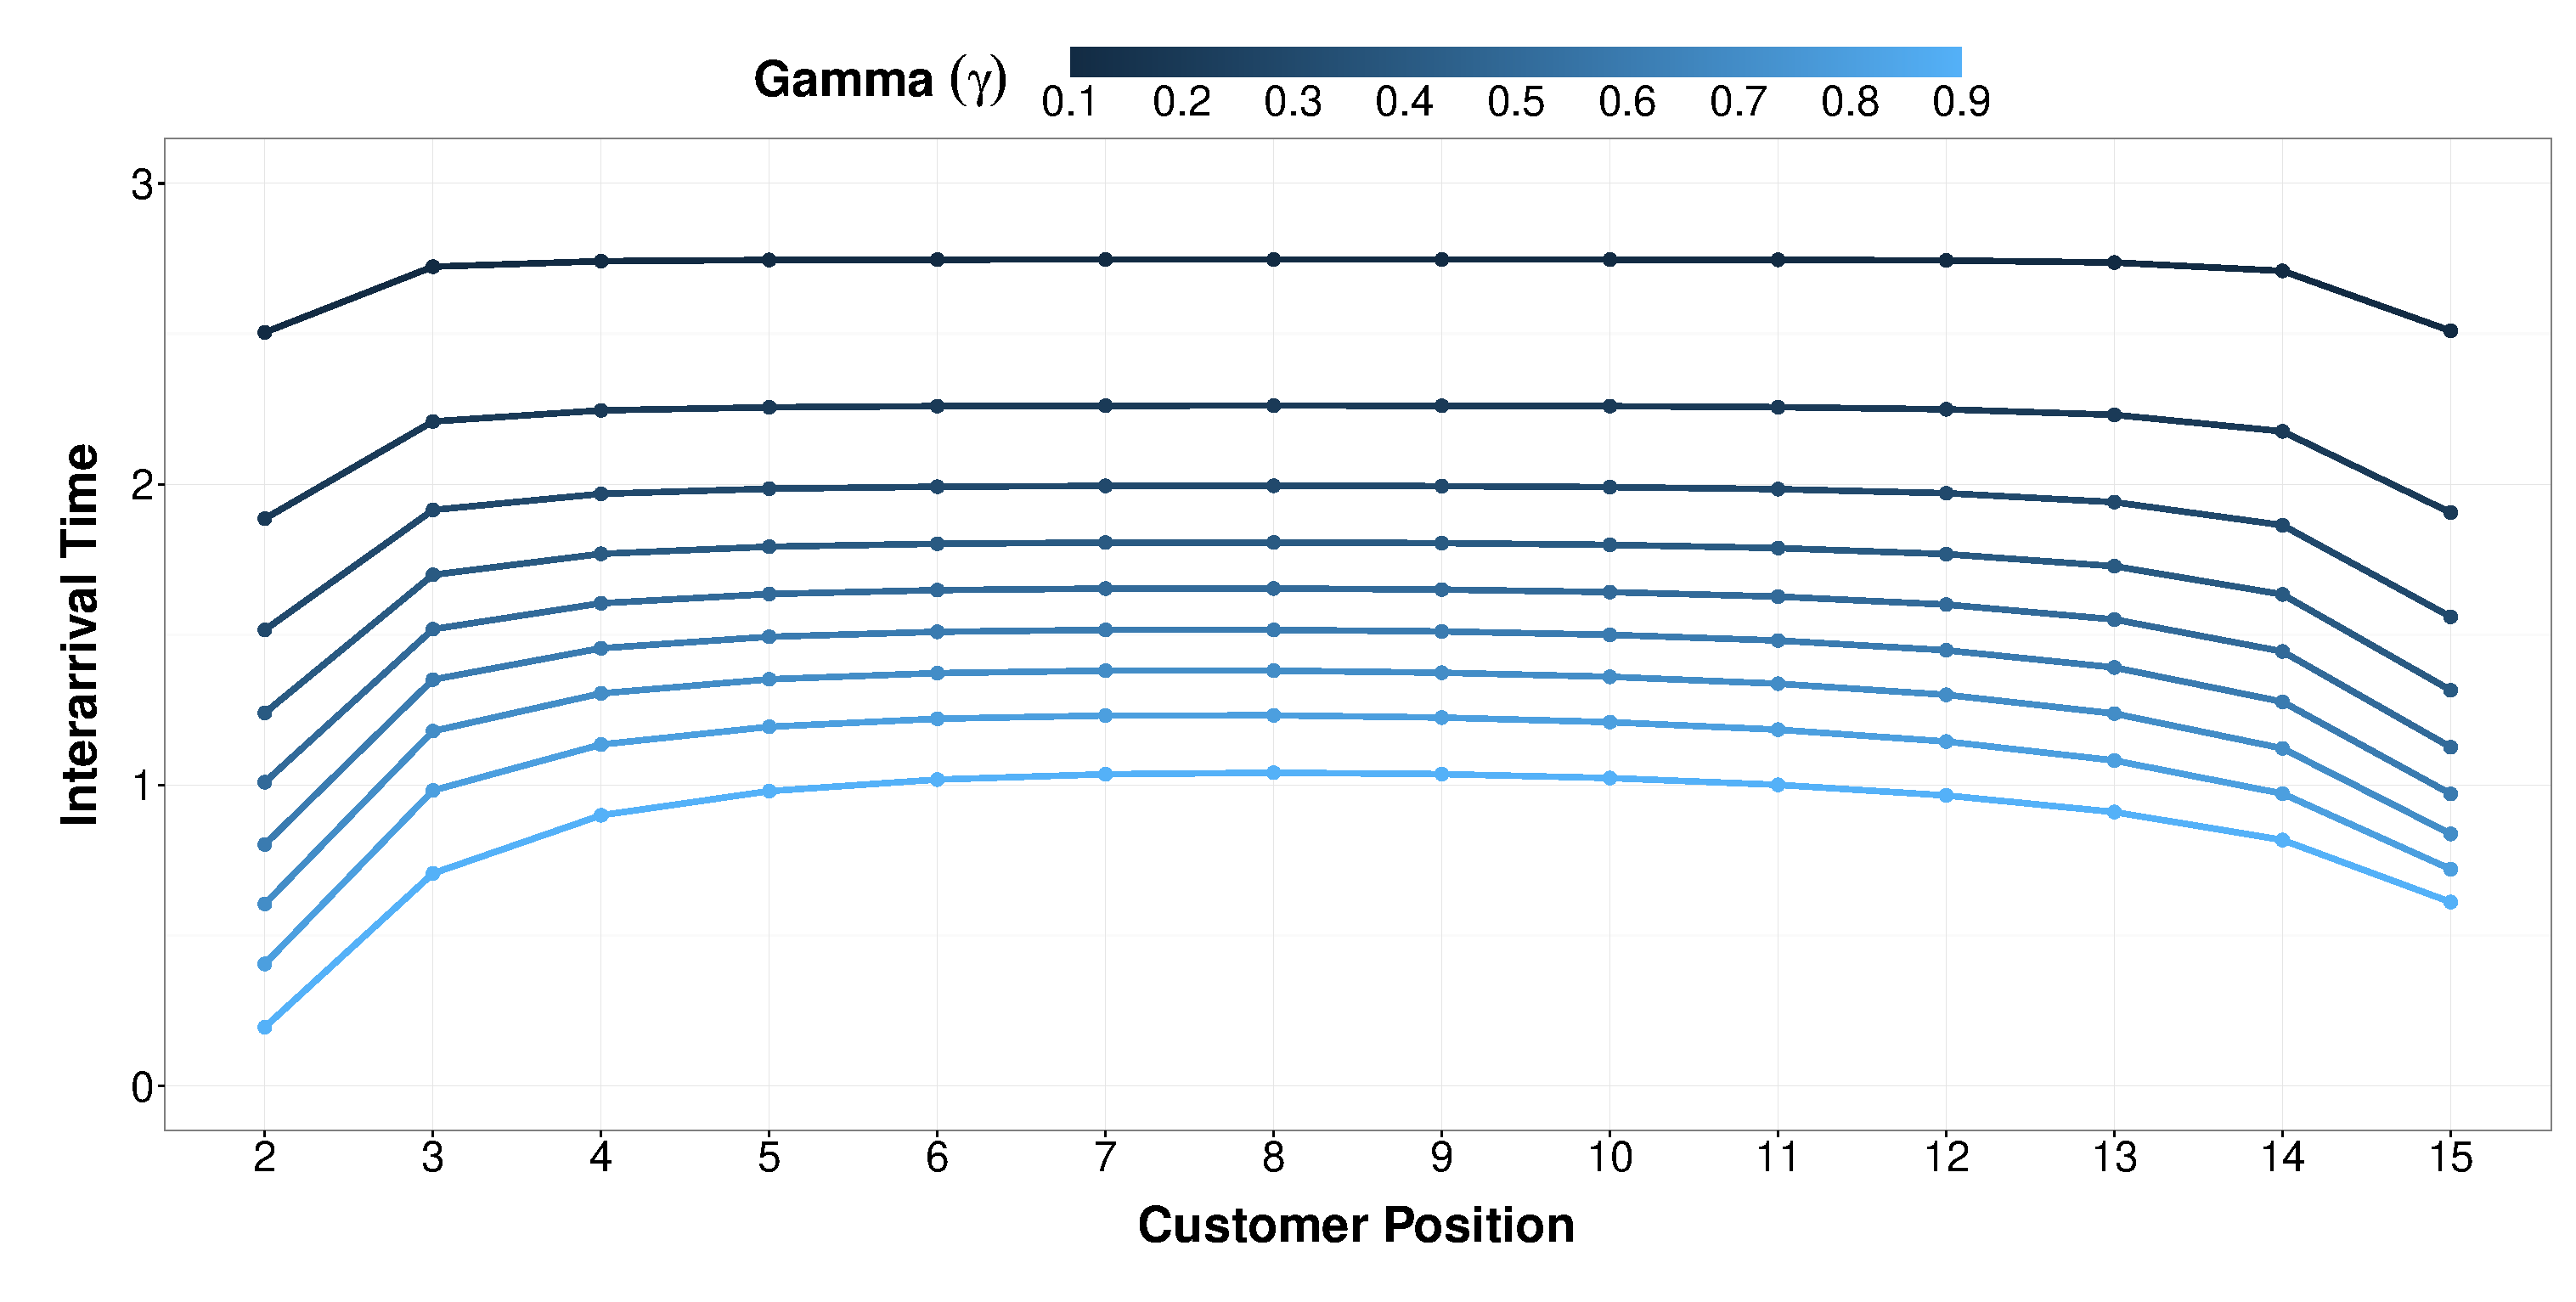
\includegraphics[width=0.85\textwidth]{Static_Line_Interarrival_Gamma.eps}
	\end{figure}

	\begin{itemize}
		\item \alert{Dome-shape}: increase for first customers, remain constant, then decrease for last few customers
		\item As relative cost of server availability time ($\gamma$) increases, customers arrive earlier
	\end{itemize}
\end{frame}

\section{Dynamic Schedules}

\begin{frame}
	\frametitle{Markov Decision Process}

	\begin{itemize}
		\item Consider the problem of scheduling $N$ customers
		\item Denote the number of customers in the system on arrival of customer $i$ by $k_{i}$
		\item $\{ k_{1}, \ldots, k_{N} \}$ is a discrete-time Markov chain
		\item On each customer's arrival, scheduler needs to schedule the arrival time of the next customer denoted by $a$
		\item Set of possible times is $\mathcal{A} = [0, \infty)$
		\item Naturally modelled as Markov decision process
	\end{itemize}
\end{frame}

\begin{frame}
	\frametitle{Expected Cost of Schedule}

	\begin{itemize}
		\item Denote the current state of $n$ customers remaining to be scheduled and $k$ customers currently in the system by $(n, k)$
		\item Expected cost of state $(n, k)$ for $n \geq 1$:
		\begin{equation*}
			C_{n}^{*} (k) = \min_{a \geq 0} C_{n} (a, k) = \min_{a \geq 0} \left[ \sum_{j = 1}^{k + 1} p_{a} (i, j) \Big( R_{a} (i, j) + C_{n - 1}^{*} (j) \Big) \right]
		\end{equation*}
	\end{itemize}
\end{frame}

\begin{frame}
	\frametitle{Erlang Distribution}

	\begin{itemize}
		\item Waiting time of customer in position $r + 1$ is sum of $r$ independent Exponential RVs with mean $\mu$
		\begin{equation*}
		 	X = \sum_{i = 1}^{r} S_{i} \sim \text{Erlang} (r, \mu)
		\end{equation*}
		\item Distribution function:
		\begin{equation*}
			F (a; r) = \mathbb{P} (X \leq x) = \begin{cases} 0 & \text{where $x = 0$} \\ 1 - \sum_{i = 0}^{r - 1} \frac{1}{i!} \left( \frac{x}{\mu} \right)^{i} \mathrm{e}^{\frac{-x}{\mu}} & \text{where $x > 0$} \end{cases}
		\end{equation*}
		\item Conditional expectation:
		\begin{equation*}
			\mathbb{E} \Big[ X \ \big| \ X \leq a \Big] = \mu r \times \frac{F (a; r + 1)}{F (a; r)}
		\end{equation*}
		\item Suppose $Y \sim \text{Exp} (\mu)$ independent of $X$ 
		\begin{equation*}
			\mathbb{E} \Big[ X \ \big| \ X \leq a, X + Y > a \Big] = \frac{a r}{r + 1}
		\end{equation*}
	\end{itemize}
\end{frame}

\section{Schedule Comparison}

\begin{frame}
	\frametitle{Expected Cost Comparison}

	\begin{itemize}
		\item 
	\end{itemize}
\end{frame}

\section{Simulation Studies}

\begin{frame}
	\frametitle{Simulation}

	\begin{itemize}
		\item 
	\end{itemize}
\end{frame}

\begin{frame}
	\frametitle{Schedule Cost}

	\begin{figure}
		\centering
		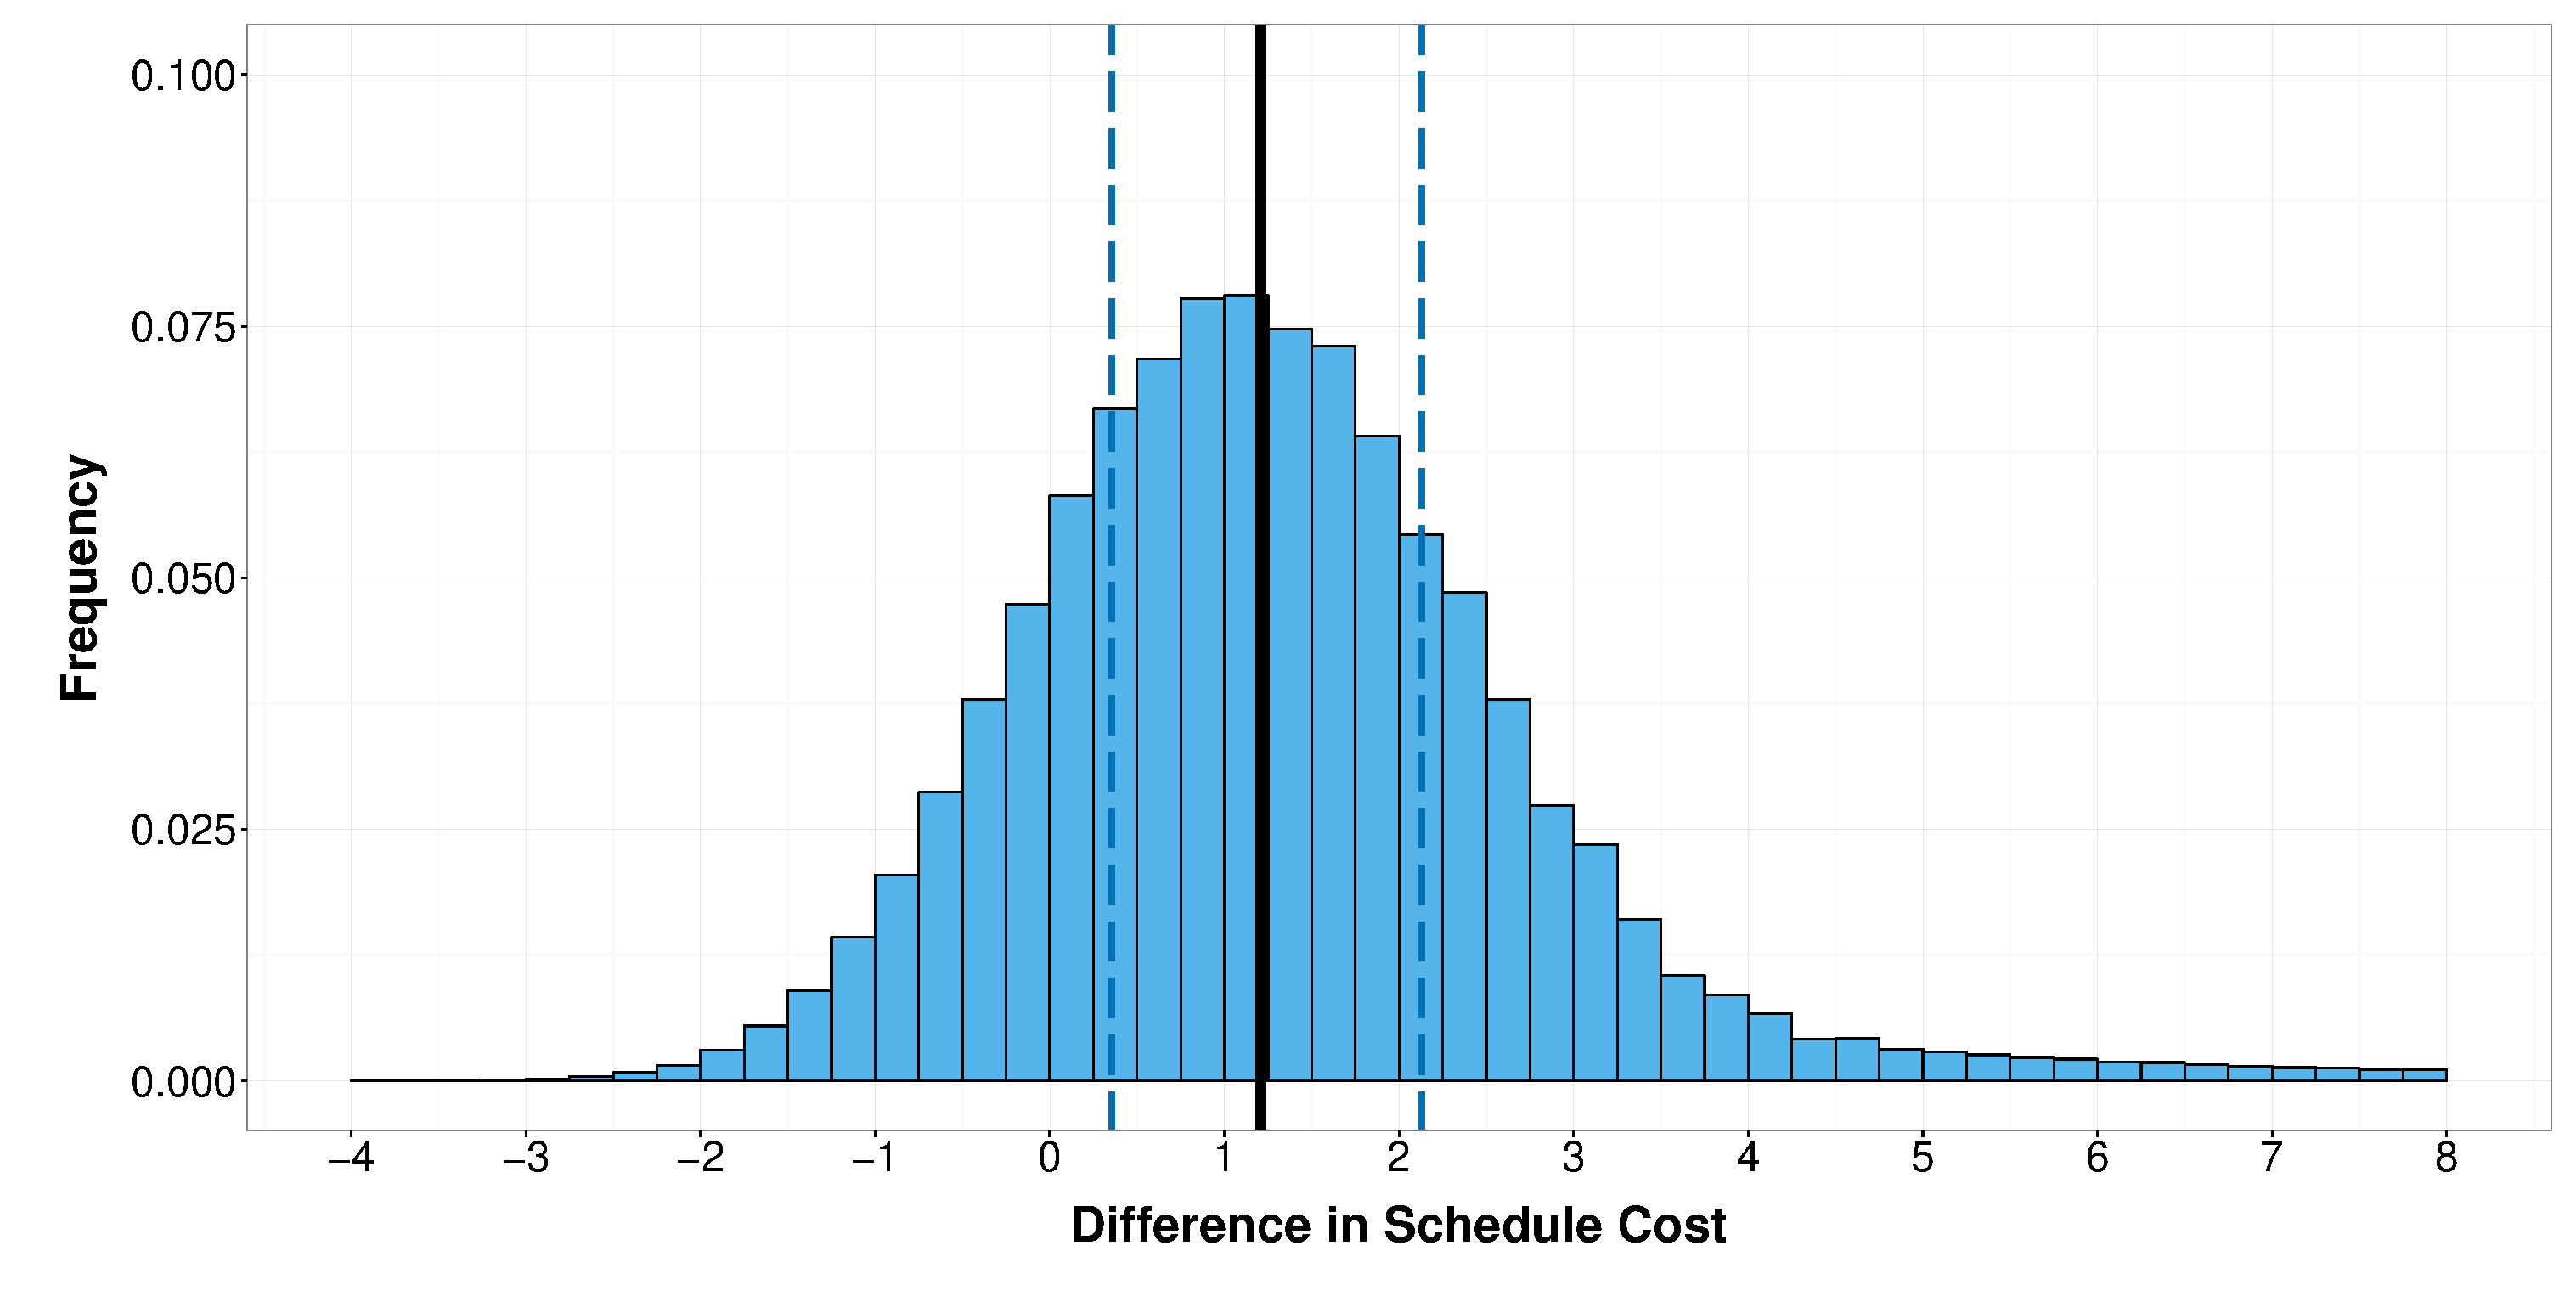
\includegraphics[width=0.85\textwidth]{Cost_Hist_Diff.eps}
	\end{figure}

	\begin{itemize}
		\item 
	\end{itemize}
\end{frame}

\begin{frame}
	\frametitle{Customer Arrival Times}

	\begin{figure}
		\centering
		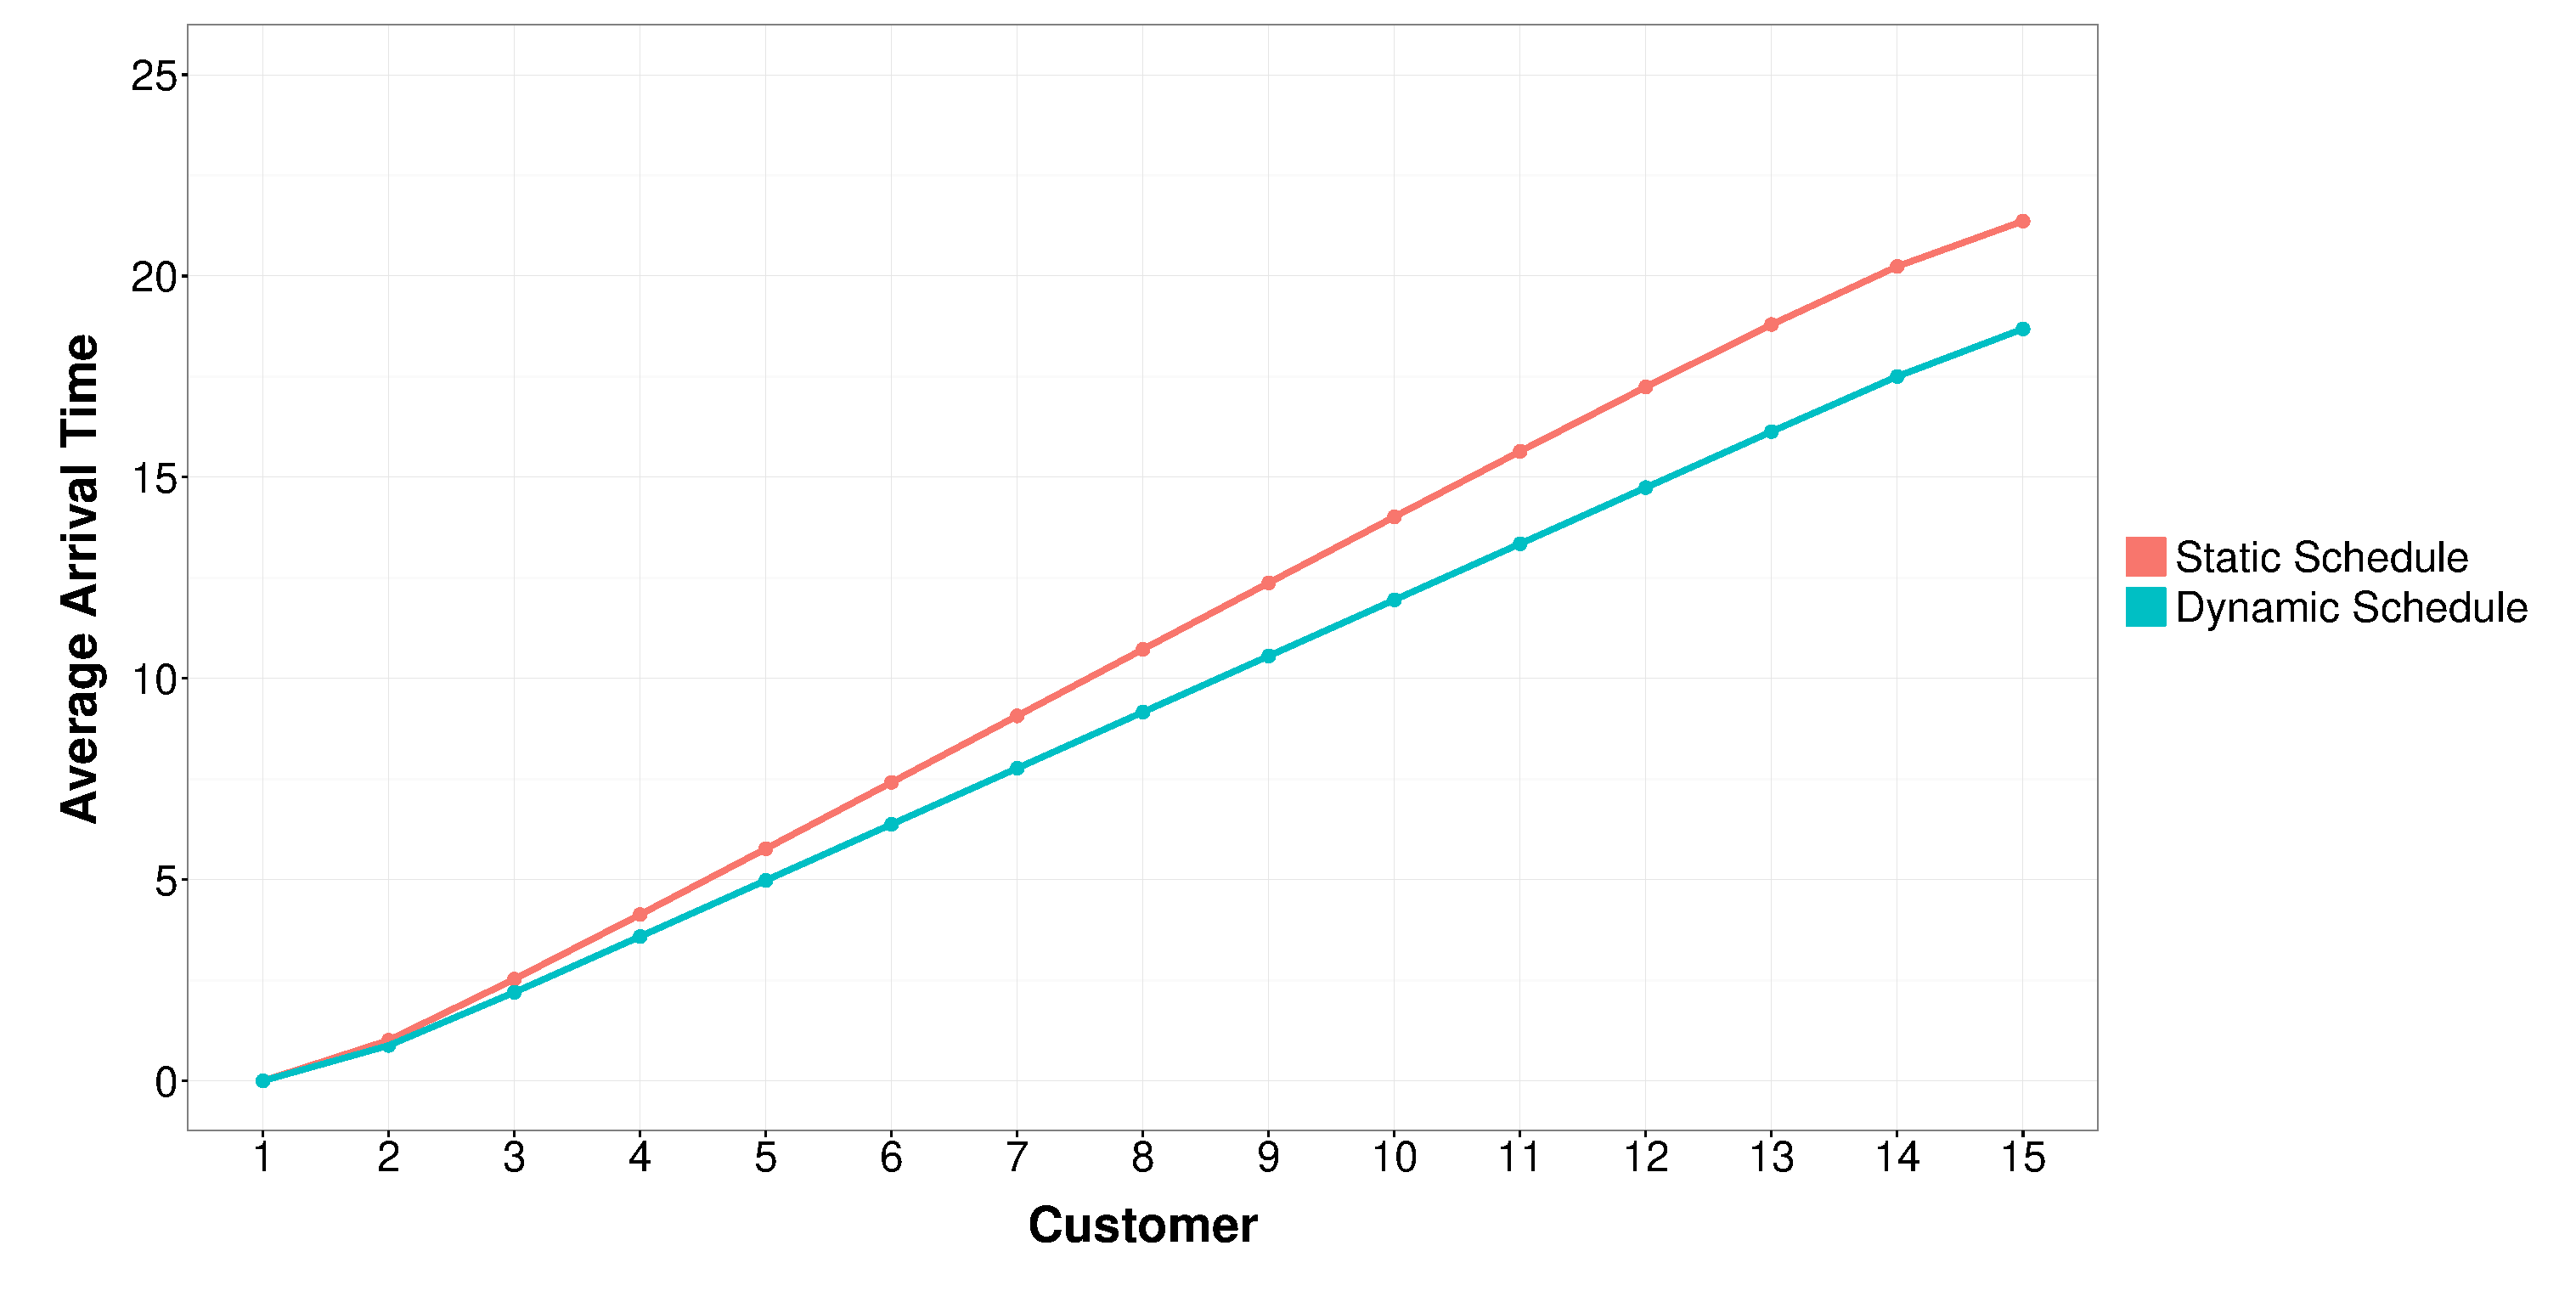
\includegraphics[width=0.85\textwidth]{AT_Line.eps}
	\end{figure}

	\begin{itemize}
		\item 
	\end{itemize}
\end{frame}

\begin{frame}
	\frametitle{Customer Waiting Times}

	\begin{figure}
			\centering
			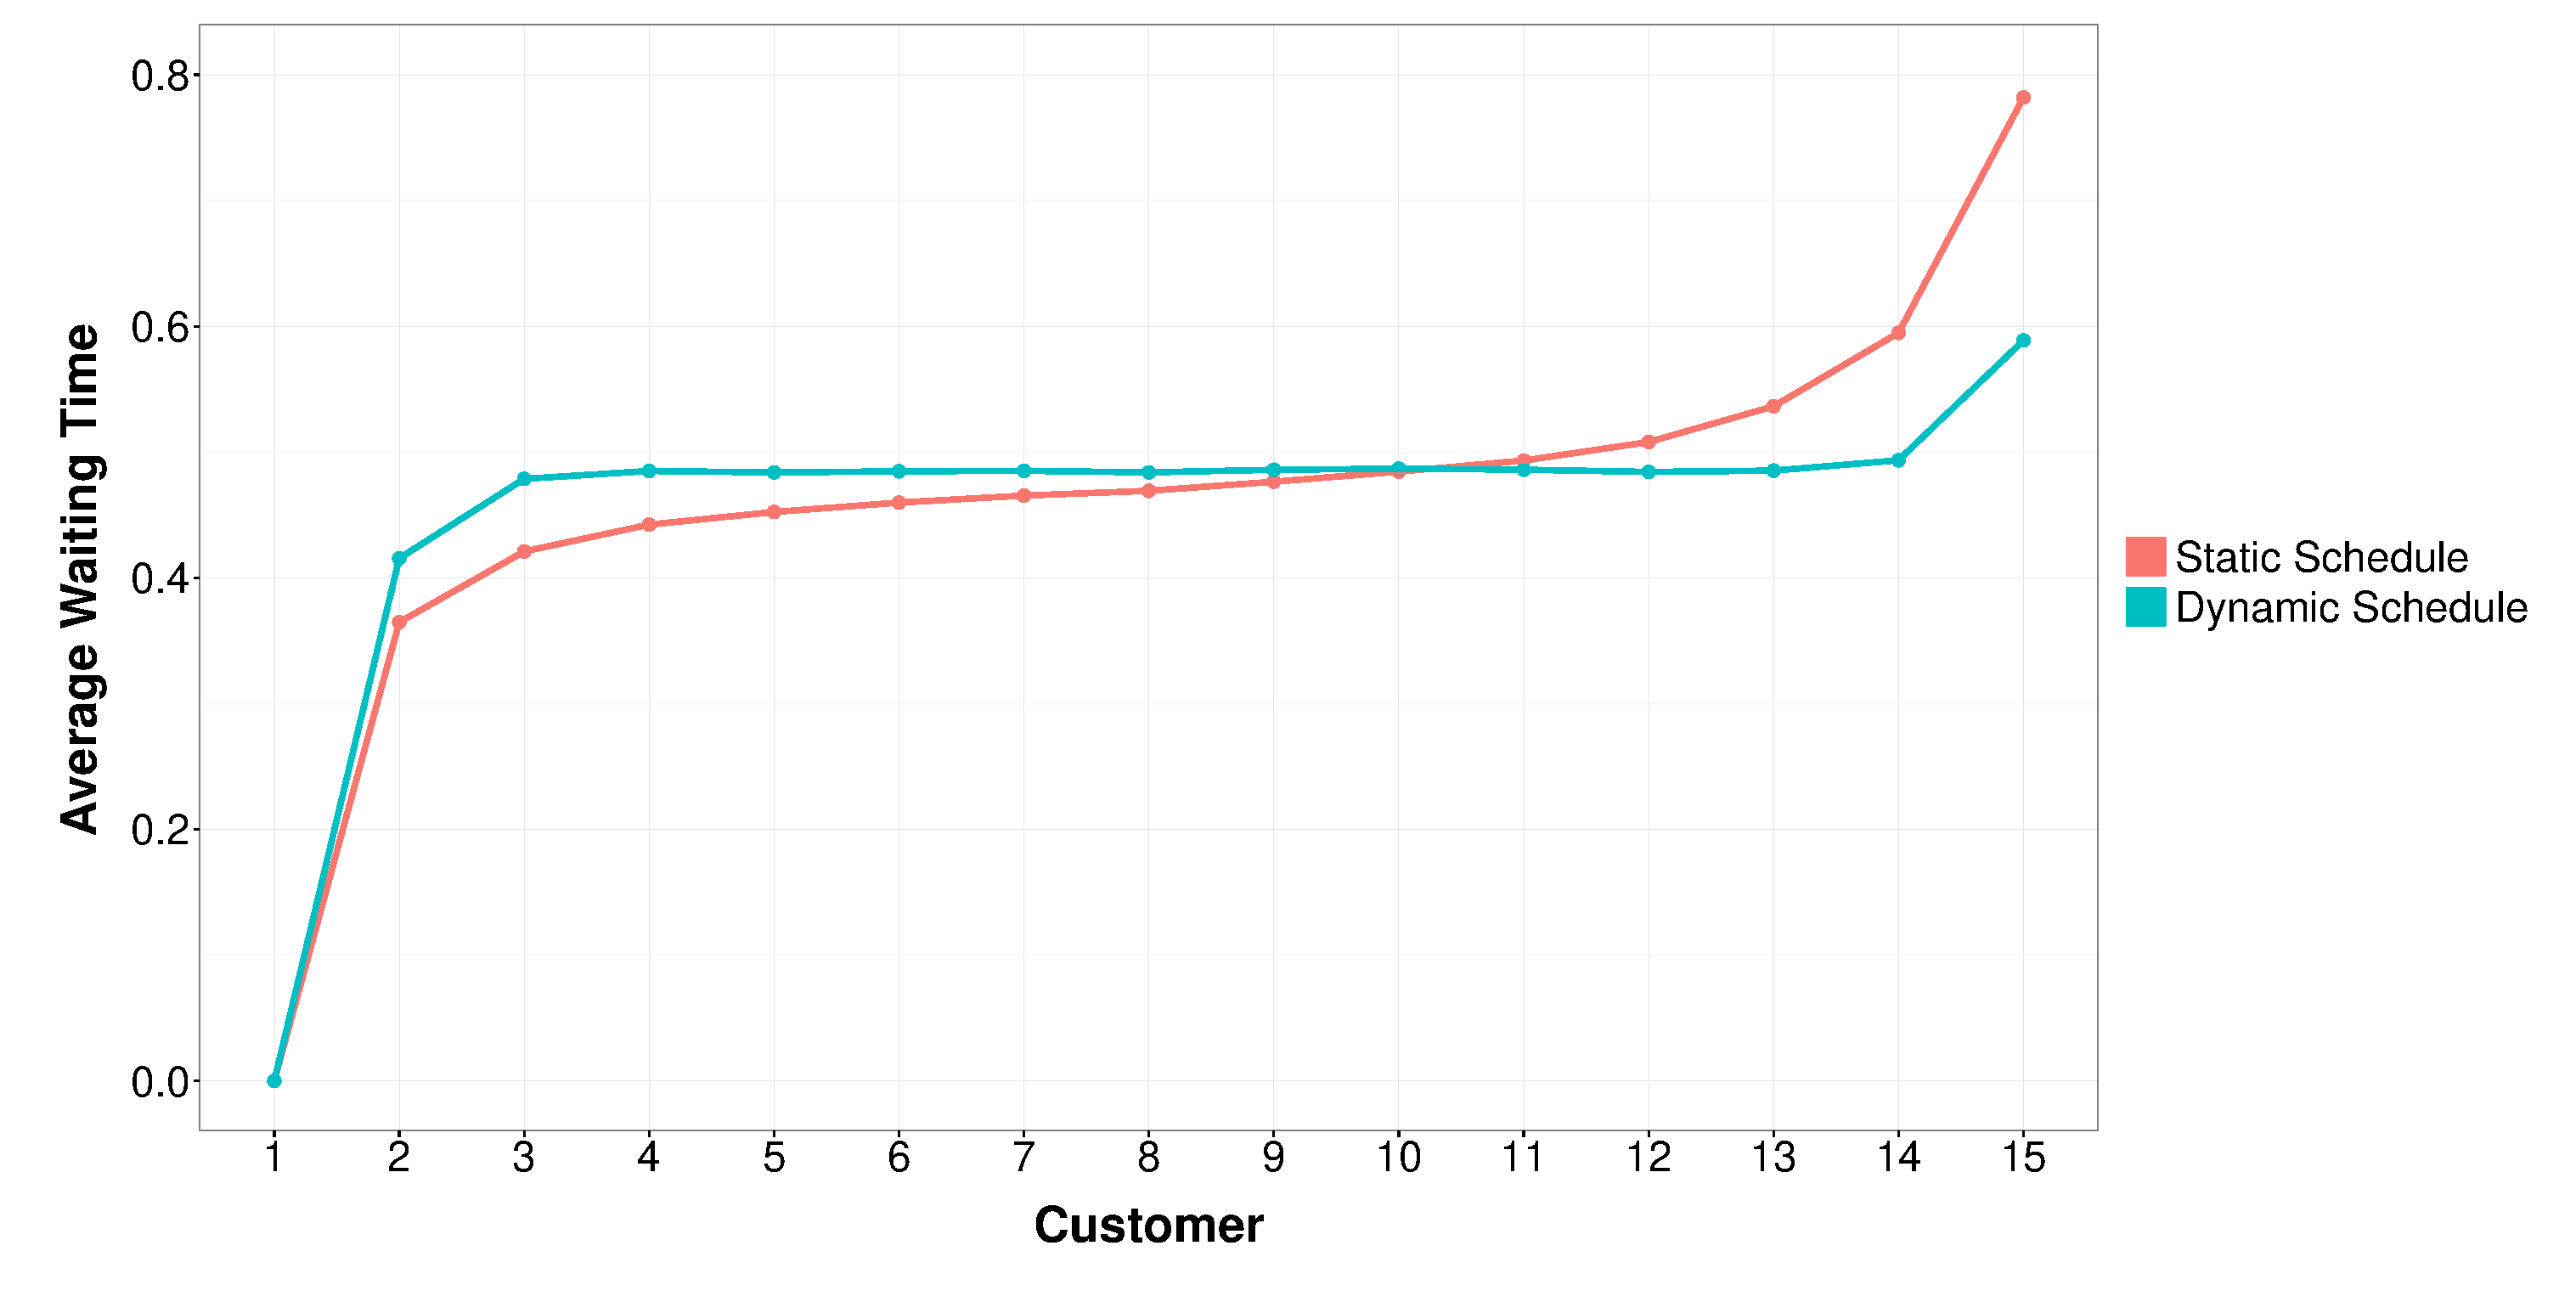
\includegraphics[width=0.85\textwidth]{WT_Line_Avg.eps}
	\end{figure}
		
	\begin{itemize}
		\item
	\end{itemize}
\end{frame}

\end{document}









































